\chapter{Eingabemethoden}
\label{cha:Eingabe}
Es gibt viele Anwendungsfälle, in denen die Interaktionen mit einem System mit den Händen nicht möglich ist. In alltäglichen Situation, wie beispielsweise beim Autofahren, bei anstrengenden und präzisen Arbeiten an Maschinen oder für Menschen mit Beeinträchtigung, sind Alternativen notwendig. Aus diesem Grund beschäftigt sich dieses Kapitel mit verschiedenen alternativen Eingabemethoden, die es auch ohne den Einsatz von den Händen ermöglichen, mit einem System interagieren zu können. Vor- und Nachteile, gesonderte Rahmenbedingungen und Einsatzgebiete werden in Kapitel~\ref{cha:Vergleich} näher erläutert.
%%%%%%%%%%%%%%%%%%%%%%% SPRACHSTEUERUNG %%%%%%%%%%%%%%%%%%%%%%%%%%%
\section{Sprachsteuerung}
Eine Alternative zur Interaktion mit den Händen stellt die Steuerung mit Hilfe der menschlichen Stimme dar. Ein Spracherkennungssystem soll im optimalen Fall das Gesprochene genau so gut erkennen und verstehen können wie ein Mensch. Da es unterschiedliche Sprachangewohnheiten, einen unterschiedlichen Dialekt und es auch syntaktische Unterschiede gibt, kann ein System an das menschliche Verstehen allerdings nur angenähert werden. Oft werden daher in der Praxis die Systeme speziell für einzelne Szenarien entwickelt bzw. angepasst. 
\newline \newline
Wird der Inhalt des Gesprochen analysiert, wird dies als Spracherkennung bezeichnet. Hier gibt es zwei Ansätze, damit das System das Gesprochene versteht:
\begin{itemize}
      \item Mustervergleich
      \item Statistische Spracherkennung
\end{itemize}
\vspace{\baselineskip}
Bei einem Mustervergleich werden die gesprochenen Wörter mit den bereits abgespeicherten Mustern und Begriffen verglichen. Jenes Wort, das dem Eingabewort am ähnlichsten ist, wird verwendet. Hingegen werden bei der statistischen Spracherkennung Beschreibungen von Lauten und Wörtern verwendet. Zusätzlich wird berechnet, welche Wortfolgen am wahrscheinlichsten sind. Hierbei werden einzelne Sequenzen des Gesprochenen verwendet und analysiert. Die Wahrscheinlichkeiten für die Wortfolgen können entweder auf einer bestehenden Statistik basieren, oder das System lernt von Eingabe zu Eingabe mit und muss für eine sichere Vorhersage im Vorhinein trainiert werden \cite{KaufmannPfisterSprache}. 
\newline \newline
%technischer aspekt
Bevor das Signal im gesamten Prozess bei dem Analyseschritt angelangt, durchläuft die Analysesequenz zuvor noch einige Prozessschritte. Wenn eine Person etwas spricht werden die analogen Wellen durch elektroakustische Wandler (zum Beispiel ein Mikrophon) in ein elektrisches Signal (Sprachsignal) umgewandelt, damit der Computer diese interpretieren und weiterverarbeiten kann. Anschließend werden auf den gespeicherten Daten verschiedenste Filter angewendet, um störende Signale, wie zum Beispiel Hintergrundgeräusche oder Pausen während des Sprechens zu entfernen. Erst dann kann im nächsten Schritt das System das Gesprochene mit Hilfe eines Mustervergleichs oder einer statistischen Spracherkennung analysieren und so den Sinn erfassen. Ist der Inhalt des Gesprochenen bekannt, kann dieser in einen Text und somit in einen Befehl umgewandelt und dadurch der Computer bzw. das Programm gesteuert werden \cite{KaufmannPfisterSprache}.
\newline \newline
Es gibt viele Faktoren, die einen Einfluss auf das Sprachsignal haben. So hat jeder Mensch neben seiner einzigartigen Stimme einen unterschiedlichen Dialekt, Sprachgewohnheiten, Emotionen in der Sprache, Pausenangewohnheiten und eine verschiedene Sprechgeschwindigkeit \cite{KaufmannPfisterSprache}. Diese Komponenten sind nicht nur wichtig für die Erkennung, was gesprochen wird, sondern viel mehr dafür, wer spricht (Sprechererkennung).
\newline \newline
%Sprechererkennung
Um festzustellen zu können welche Person gerade spricht, muss es Referenzdaten im System geben, die mit dem aktuellen Signal verglichen werden können. Dies geschieht entweder, wenn die Person ein bestimmtes Signalwort spricht, das mit dem abgespeicherten Wort verglichen wird, oder wenn das Sprachsignal lange genug ist, kann auf Grund von statistischen Merkmalen wie \zB Stimmfarbe oder Sprechgeschwindigkeit eine Übereinstimmung gefunden werden \cite{KaufmannPfisterSprache}. 
\newline \newline
%Interaktion!
Kommunikation durch Sprache ist eines der leichtesten, wenn nicht sogar das intuitivste Mittel zur Verständigung. Daher sollte auch die Interaktion mit einem Computer diesem hohen Standard entsprechen. Allerdings ist im Gegensatz zur gewohnten Face-to-Face-Kommunikation das Gegenüber im Bezug auf Spracherkennung kein intelligenter Gesprächspartner. Ein Computer kann nur schwer lange und komplizierte Sätze und Gedankengänge mitverfolgen und daraus schlecht eine Kernaussage ziehen. Daher muss dem System verständlich gemacht werden, wann es zuhören soll \cite{SpeechInteraction}.
Zwei gängige Methoden für den Start zur Interaktion sind:
\begin{itemize}
      \item das Drücken einer Starttaste
      \item das Aussprechen eines Aktivierungswortes
\end{itemize}
\vspace{\baselineskip}
Weil das Drücken eines Startknopfes die Hilfe der Hände benötigt, steht im Kontext dieser Arbeit das Aussprechen eines Aktivierungswortes zum Start der Interaktion im Vordergrund. Durch das Wort 'Alexa' wird beispielsweise Amazon Echo%
\footnote{https://www.amazon.com/Amazon-Echo-Bluetooth-Speaker-with-WiFi-Alexa/dp/B00X4WHP5E}
%
aktiviert. Bei Amazon Echo handelt es sich um ein Sprachinteraktionssystem, das beispielsweise Musik abspielen, den Einkauf bestellen oder auch Nachrichten und Wetterbeiträge zur Verfügung stellen kann.
Im Gegensatz zur Benutzung von Amazon Echo, muss bei der Sprachsteuerung von Apple (Siri)%
\footnote{https://www.apple.com/ios/siri/}
%
 das System erst auf die eigene Stimme eingestellt, also kalibriert werden. Das Aktivierungswort 'Hey Siri' muss drei Mal einzeln und zwei Mal in einem Satz eingesprochen werden, damit diese Funktion beispielsweise am iPhone freigeschaltet wird. Anschließend können ebenfalls Wetter oder Nachrichtendaten abgefragt werden, aber auch Anrufe oder Nachrichten können mit Hilfe der Stimme getätigt werden. 
\newline \newline
Sobald das System bereit ist die Eingabe aufzunehmen, muss beachtet werden, dass laut und deutlich gesprochen wird, keine zu große Distanz zum Mikrophon besteht und dass nicht zu schnell gesprochen wird.
\newline \newline
Zusammenfassend lässt sich sagen, dass die Sprachinteraktion mit dem Computer aus Benutzersicht noch einige Verbesserung braucht, damit die Bedienung natürlicher und intuitiver wird und der einer Face-to-Face-Kommunikation näher kommt.

%%%%%%%%%%%%%%%%%%%%%%% AUGENSTEUERUNG %%%%%%%%%%%%%%%%%%%%%%%%%%%
\section{Augensteuerung}
\label{cha:Augensteuerung}

Eine weitere alternative Interaktionsmöglichkeit stellt die Steuerung mit Hilfe der Augen dar. Eye-Tracking-Systeme werden verwendet, um die Augenbewegungen zu identifizieren. Parallel dazu wandelt eine Software die Augenbewegungen in einen Mauszeiger um, um so mit dem System interagieren zu können. 
\newline \newline
Um die Augenbewegungen nachvollziehen zu können, werden sowohl ein Infrarotlichtstrahl, als auch eine Videokamera auf das Auge fokussiert. Eine Software analysiert die Bewegungen im Hintergrund und erkennt, wo der Fokus auf dem Bildschirm liegt. Für die Umrechnung ist außerdem wichtig, dass die Position des Kopfes vom Interaktionssystem erkannt wird \cite{NielsenPernice}.
\newline \newline
Die Teilbereiche des Auges bzw. des menschlichen Sehens, die für die Augensteuerung relevant sind, sind das periphere und foveale Sehen. Das foveale Sehen beinhaltet jenen Teil, den das menschliche Auge als scharfen Bildausschnitt wahrnimmt, also auf welchen Ausschnitt es fokussiert. Hingegen enthält das periphere Sehen den Großteil unser Sehwahrnehmung. Dies beinhaltet jene Bereiche, die nicht fokussiert sind \cite{NielsenPernice}. Daher ist das foveale Sehen für die Augensteuerung relevant.
\newline \newline
Nielsen und Pernice \cite{NielsenPernice} unterscheiden beim menschlichen Sehen zusätzlich zwischen Fixation und Sakkaden. Das menschliche Auge bewegt sich nicht kontinuierlich, sondern ein Blick setzt sich aus schnellen Bewegungen mit Pausen dazwischen zusammen. Dies geschieht so schnell, dass es im Alltag nicht bewusst wahrgenommen wird. Wenn das Auge auf einem bestimmten Punkt ruht spricht man von Fixation. Die schnellen Zwischenbewegungen von einer Fixation zur nächsten werden Sakkaden genannt. Die Schwierigkeiten der Eye-Tracking-Systeme und der Augensteuerungssoftware bestehen darin, diese Fixationen zu erkennen, da diese meist zwischen einer hundertstel und einer zehntel Sekunde liegen \cite{NielsenPernice}.
%abbildung 2
\begin{figure}
\centering
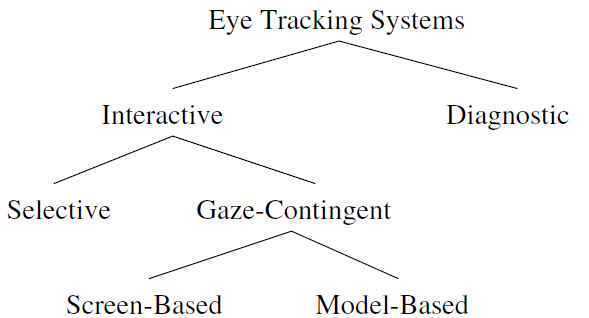
\includegraphics[width=.7\textwidth]{eyeTrackingSystems}
\caption{Hierachie von Eye-Tracking-Systemen \cite{Duchowski}.}
\label{fig:eyeTrackingSystems}
\end{figure}
\newline \newline
Wie in Abb.~\ref{fig:eyeTrackingSystems} dargestellt, unterscheidet Duchowski \cite{Duchowski} zwischen interaktiven und diagnostischen Systemen. Da bei diagnostischen Systemen keine direkte Interaktion stattfindet, sondern die Augenbewegungen aufgezeichnet und im Nachhinein ausgewertet werden, sind für die Analyse von Interaktionsmöglichkeiten ausschließlich interaktive Systeme relevant. 
\newline \newline
Interaktive Systeme lassen sich wiederum in zwei Bereiche teilen. Selektive Systeme benutzen den Blickpunkt als analoges Eingabeelement, während Blickkontingentsysteme für die Darstellung von komplexen Displays verwendet werden. 
\newline \newline
Abgesehen davon, wie die Daten aufgezeichnet werden bzw. was aufgezeichnet wird, gibt es eine Unterscheidung zwischen den verschiedenen Eye-Tracking-Systemen. Diese können in intrusive und nicht-intrusive Systeme unterteilt werden. Intrusive Eye-Tracker haben einen direkten Kontakt mit den Anwendern (\zB durch Kontaktlinsen). Nicht-intrusive Eye-Tracking-Systeme hingegen messen die Blicke mit Hilfe einer oder mehrerer Kameras. 
\newline \newline
In der Praxis werden eine Vielzahl verschiedenster Eye-Tracking-Systeme als Basis für die Augensteuerung verwendet. Die Unternehmen Tobii%
\footnote{http://www.tobii.com/group/}
%
und SensoMotoricInstruments (SMI)%
\footnote{https://www.smivision.com/}
%
sind Spitzenreiter auf dem Gebiet des Eye-Tracking und verfügen über eine umfangreiche Produktpalette bzw. vielfältige Anwendungsgebiete. 
\begin{figure}
\centering\small
\setlength{\tabcolsep}{0mm}	% alle Spaltenränder auf 0mm
\begin{tabular}{c@{\hspace{-15mm}}c} % mittlerer Abstand = 12mm
  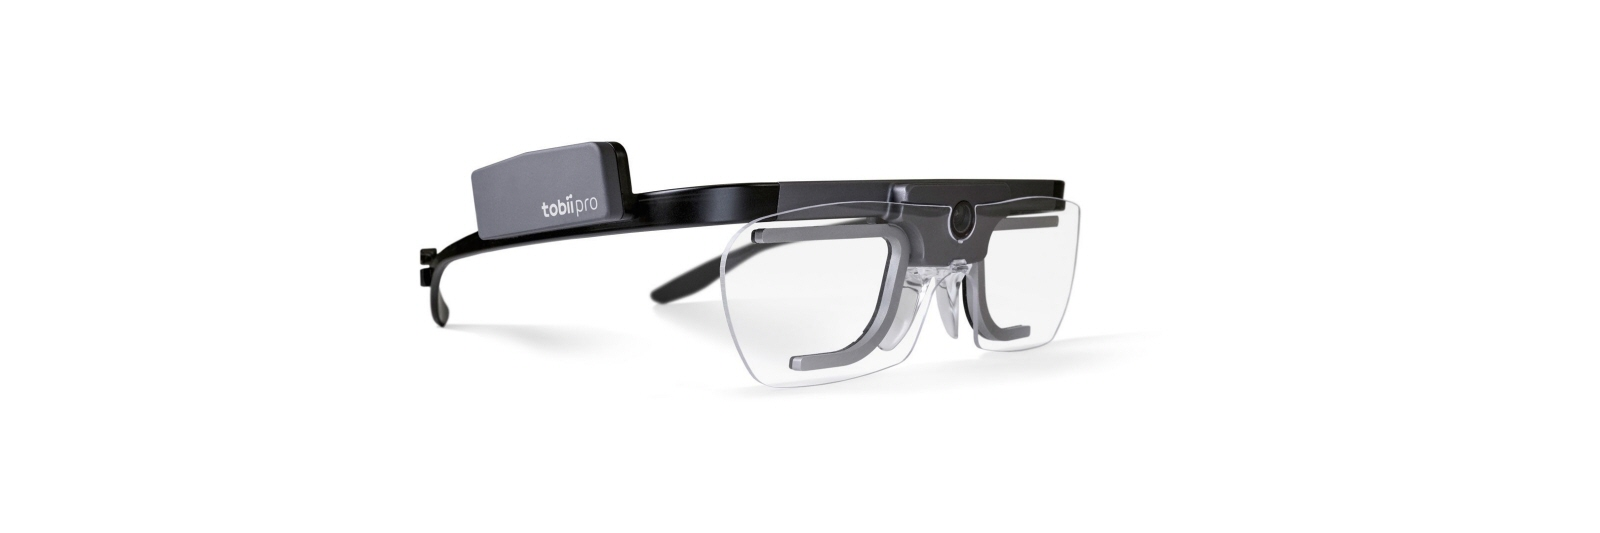
\includegraphics[width=.6\textwidth]{TobiiPro_Glasses} &
  
\includegraphics[width=.6\textwidth]{Tobii_Spectrum}
\\
  (a) & (b)
\\[4pt]	%vertical extra spacing (4 points)
  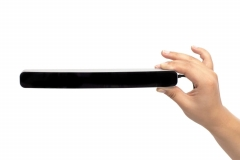
\includegraphics[width=.36\textwidth]{SMIRED}
\\
  (c)
\end{tabular}
%
\caption{Übersicht über die Eye-Tracking-Systeme von Tobii und SMI \newline
(a)~Tobii Pro Glasses 2 \cite{TobiiGlasses}, (b)~Tobii Pro Spectrum \cite{TobiiSpectrum} und (c)~SMI Red250mobile \cite{SMIRED}.}
\label{fig:Tobii}
\end{figure}
\newline \newline
In Abb.~\ref{fig:Tobii}(a) ist die tragbare Eye-Tracking-Brille Tobii Pro Glasses 2 zu sehen. Diese ist so gestaltet worden, um ein möglichst natürliches Nutzungsverhalten zu erzielen. Es müssen keine Voreinstellungen vorgenommen werden, die Brille kann sofort benutzt werden. Bei Tobii Pro Spectrum (Abb.~\ref{fig:Tobii}(b)) handelt es sich um ein nicht-intrusives System, das die Blickdaten mit einer Geschwindigkeit von bis zu 600 Hz aufnimmt. Das Unternehmen SMI hat, wie in Abb.~\ref{fig:Tobii}(c) zu sehen ist, ein mobiles Eye-Tracking-System entwickelt, das die Bewegungen mit bis zu 250 Hz aufzeichnen kann. Alle diese Systeme verwenden das Prinzip von Fixation und Sakkaden des Auges, um die Augenbewegungen nachvollziehen zu können. Damit nicht nur die Augenbewegungen aufgezeichnet werden, sondern eine Interaktion stattfinden kann, müssen diese Systeme in Kombination mit einer Software eingesetzt werden, die die Blicke in Mausbewegungen o.ä. umwandelt.
\newline \newline
Bevor ein Benutzer mit Hilfe der Augen beispielsweise eine Bildschirmtastatur bedien kann, muss das System bzw. die Software erst auf den Anwender eingestellt werden. Bei der Kalibrierung tauchen am Bildschirm nacheinander Symbole auf, die fixiert werden müssen. Dadurch können der Blickwinkel und der Augenabstand vermessen werden um eine optimale Interaktion zu erreichen. Bei der eigentlichen Anwendung erkennt das System dann, wenn der Blick auf einem Punkt länger verharrt, also scharf stellt. Verharrt der Blick also länger auf einem Buchstaben der Tastatur, wird dies als Mausklick gewertet und der Buchstabe oder das Symbol ausgewählt. Am Beispiel von Seetech von Humanelektronik%
\footnote{http://humanelektronik.de/}
%
beträgt die Fixationszeit etwa 0.5 bis 1.5 Sekunden \cite{SEETECH}.
\newline \newline \newline
Zusammenfassend kann gesagt werden, dass für die Interaktion mit einer Anwendung bzw. einem System interaktive Eye-Tracking-Systeme für die Nachvollziehbarkeit der Augenbewegungen und zusätzlich eine Software für die Umrechnung in Mausbewegungen relevant sind. Nach einer kurzen Kalibrierung können durch Fixation einzelne Elemente auf dem Bildschirm ausgewählt und auf Grund der Fixationszeit in einen Mausklick umgewandelt werden.

%%%%%%%%%%%%%%%%%%%%%%% Gestensteuerung %%%%%%%%%%%%%%%%%%%%%%%%%%%
\section{Gestensteuerung}

Eine weitere Alternative zur Interaktion mit den Händen stellt die Gestensteuerung dar. Mit Hilfe von Gesten kann eine Handlung mit verschiedenen Teilen des Körpers (\zB den Händen, Füßen, Kopf) zum Ausdruck gebracht werden. In diesem Abschnitt bezieht sich die Gestensteuerung auf alle Körperteile ausschließlich der Hände. In der Literatur werden Gesten unterschiedlich definiert, in diesem Zusammenhang versteht man unter einer Geste \cite{PreimDachselt}:
\begin{quote} ...die Bewegung von Fingern, Händen und Armen - oder auch weiterer Körperteile, wie Kopf, Augen und Lippen - aufgrund einer kommunikativen Absicht. Damit enthält die Bewegung als solche signifikante Informationen, die an den Computer übermittelt werden sollen. \end{quote}
In diesem Abschnitt werden Kinn-, Mund-, Kopf- sowie Fußsteuerung näher erläutert. 
%
%
%%%%%%%%% Kinnsteuerung %%%%%%%%%
\subsection{Kinnsteuerung}
\label{cha:Kinnsteuerung}

Bei der Kinnsteuerung werden mit Hilfe des Kinns Bewegungen ausgeführt, um mit einem System interagieren zu können. Die unterschiedlichen Möglichkeiten werden anhand der nachfolgenden Beispiele erklärt.
%
\begin{figure}
\centering\small
\setlength{\tabcolsep}{0mm}	% alle Spaltenränder auf 0mm
\begin{tabular}{c@{\hspace{15mm}}c} % mittlerer Abstand = 12mm
  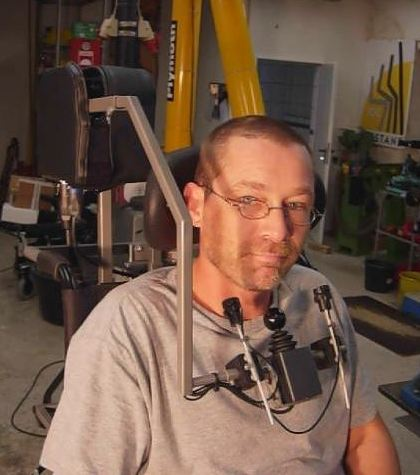
\includegraphics[width=.3\textwidth]{moso_kinn} &
  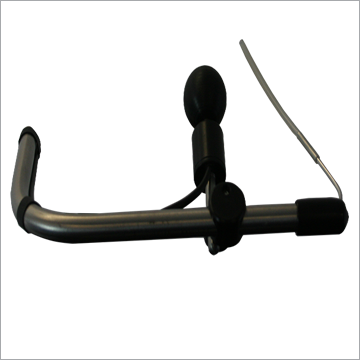
\includegraphics[width=.3\textwidth]{smilesmart_kinn}
\\
  (a) & (b)
\\[5pt]	%vertical extra spacing (4 points)
  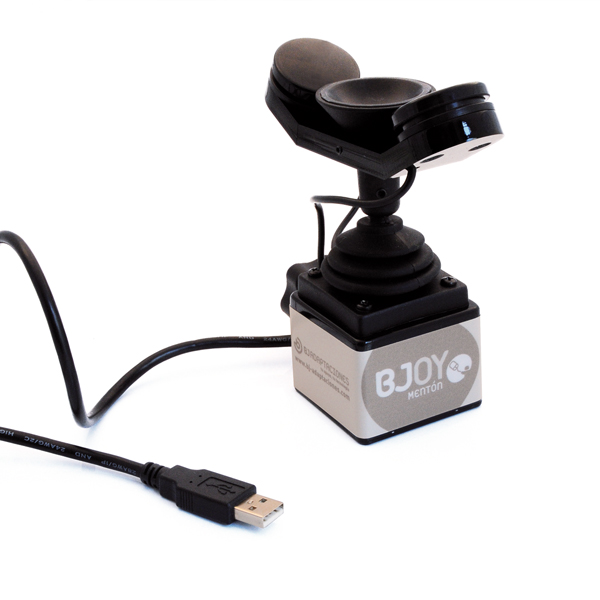
\includegraphics[width=.3\textwidth]{sensory_kinn}
\\
  (c)
\end{tabular}
%
\caption{(a)~Moso® Kinnsteuerung \cite{MOSO}, (b)~Smile Smart Kinnsteuerung \cite{SMILESMART} und (c)~Sensory Kinnsteuerung \cite{SENSORY}.}
\label{fig:kinn}
\end{figure}
\newline \newline
Wie in Abb.~\ref{fig:kinn}(a) zu sehen ist verwendet das Unternehmen moso®%
\footnote{http://www.moso-gmbh.de/}
%
einen Joystick und zwei Tasten für die Interaktion. Um einen angenehmen Umgang zu gewährleisten, ist der Joystick mit einem kleinen weichen Ball ausgestattet. Zwei Tasten sind links und rechts des Joysticks angebracht. Der Joystick kann sich in alle Himmelsrichtungen bewegen und kann so entweder als Mauszeiger, oder zur Steuerung eines Rollstuhls genutzt werden. Die beiden Tasten können als linke und rechte Maustaste verwendet werden \cite{MOSO}.
\newline
Abb.~\ref{fig:kinn}(b) zeigt die Version der Firma Smile Smart Technology%
\footnote{https://smilesmart-tech.com/}
%
. Diese besteht aus einem Mini Rollstuhl Joystick, der auf einer schwenkbaren Halterung montiert ist \cite{SMILESMART}.
\newline
Die Kinnsteuerung des Unternehmens Sensory Guru%
\footnote{http://www.sensoryguru.com/}
%
weist im Vergleich zu den anderen beiden keinen Ball auf. Wie in Abb.~\ref{fig:kinn}(c) dargestellt, weist der Joystick eine Mulde für das Kinn auf. Mit einer Bewegung nach links oder rechts können die beiden äußeren Sensoren aktiviert werden. Das Kinn muss dabei im ständigen Kontakt mit dem Ball bzw. Joystick stehen \cite{SENSORY}. 
\newline
Durch eine stärke Kinnbewegung nach links bzw. rechts oder über zusätzlich angebrachte Tasten an der Steuerung, kann durch ein Menü navigiert werden. Des Weiteren können auch andere Symbole auf einem Bildschirm ausgewählt werden. Durch die Bedienung des Joystickelementes kann der Benutzer beispielsweise die Bewegungen einer Computermaus nachahmen \cite{MOSO} \cite{SENSORY}. 
\newline
Dies kann je nach Ausführung der Steuerung verschieden viele Freiheitsgrade beinhalten. Freiheitsgrade bzw. Degrees of Freedom (DoF) bezeichnen die Bewegungsfreiheit eines Körpers.
\newline \newline
Abb.~\ref{fig:6DoF} zeigt sechs Freiheitsgrade bzw. sechs verschiedene Bewegungsrichtungen \cite{6DoF}:
\begin{itemize}
      \item Hinauf und hinunter (Up and Down)
      \item Links und rechts (Left and Right)
			\item Vorwärts und Rückwärts (Forward and Back)
			\item Kippen entlang der X-Achse (Roll)
      \item Kippen entlang der Y-Achse (Pitch)
			\item Kippen entlang der Z-Achse (Yaw)
\end{itemize}
%
\vspace{\baselineskip}
Bei der Kinnsteuerung von Mosco werden fünf Freiheitsgrade ermöglicht, das bedeutet dass der Joystick in alle Richtungen bewegt und geneigt werden kann, das Kippen entlang der Z-Achse ist allerdings nicht möglich. Bei der Ausführung des Unternehmens Sensory sind nur vier Freiheitsgrade möglich, da der Joystick nicht in Z-Richtung bewegt werden kann. 
Wie stark der Joystick in die bestimmte Richtung gedrückt werden muss, um eine gewisse Bewegung zu erzeugen, kann an den jeweiligen Benutzer angepasst werden, um eine optimale Interaktion zu erreichen.
%
\begin{figure}
\centering
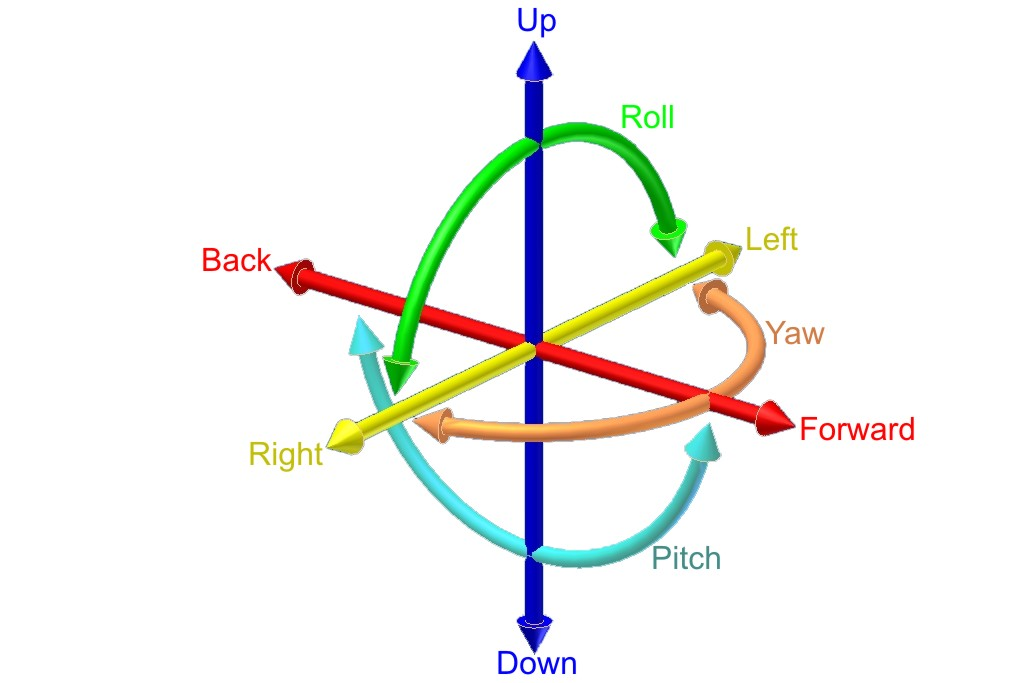
\includegraphics[width=.68\textwidth]{6DoF}
\caption{Sechs Freiheitsgrade \cite{6DoFPic}.}
\label{fig:6DoF}
\end{figure}
%
%

%%%%%%%%% Mundsteuerung %%%%%%%%%
\subsection{Mundsteuerung}

Das Prinzip der Mundsteuerung funktioniert ähnlich wie die der Kinnsteuerung. Durch die verschiedenen Interaktionsmöglichkeiten, die durch den Einsatz des Mundes durchführbar sind, wird versucht, eine Interaktion, beispielsweise mit einem Computer, möglich zu machen.
\newline \newline
Bei der in Abb.~\ref{fig:mund}(a) gezeigten Mundsteuerung handelt es sich um die IntegraMouse Plus, die das Unternehmen LIFEtool%
\footnote{http://www.lifetool.at/startseite/}
%
entwickelt hat. Durch das Bewegen des Mundstückes der IntegraMouse Plus kann die Richtung bzw. der Cursor verändert werden. Zusätzlich zur reinen Steuerung durch eine Geste kann durch Pusten ein Rechtsklick und durch Nippen ein Linksklick erzeugt werden \cite{INTEGRA_VIDEO}.
\newline \newline
Ähnlich wie bei der IntegraMouse Plus wird bei dem mundgesteuerten Gamecontroller der Firma QuadStick%
\footnote{http://www.quadstick.com/}
%
, der in Abb.~\ref{fig:mund}(b) zu sehen ist, ebenfalls Nippen, Pusten und Bewegungen des Mundes zur Interaktion verwendet. Dieses Modell besitzt allerdings vier Nipp- bzw. Pustsensoren, um einen regulären Gamecontroller besser imitieren zu können. Die drei zusätzlichen Sensoren können individuell angepasst und beispielsweise als Shortcuts für bestimmte Computerspiele verwendet werden. Ein Shortcut bzw. ein Sensor beinhaltet eine Reihenfolge von Klick- und Bewegungsabläufen, die als Kombination dargestellt werden \cite{QUADSTICK}. In einem gewöhnlichen Computersetting könnten die Shortcuts beispielsweise als Scrollbewegung verwendet werden, die ansonsten durch das Hinauf- oder Hinunterbewegen mit zwei Fingern am Touchpad funktionieren.
\newline \newline
Bei beiden Steuerungen ist vor der Benutzung keine Kalibrierung notwendig. Am Computer muss lediglich ein USB-Stick angeschlossen werden, der die Mundsteuerung per Bluetooth-Verbindung ermöglicht. 

\begin{figure}
\centering\small
\setlength{\tabcolsep}{0mm}	% alle Spaltenränder auf 0mm
\begin{tabular}{c@{\hspace{15mm}}c} % mittlerer Abstand = 12mm
  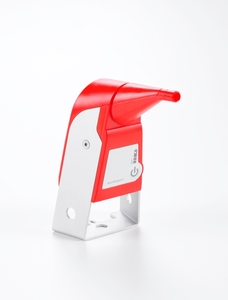
\includegraphics[width=.29\textwidth]{IntegraMouse} &
  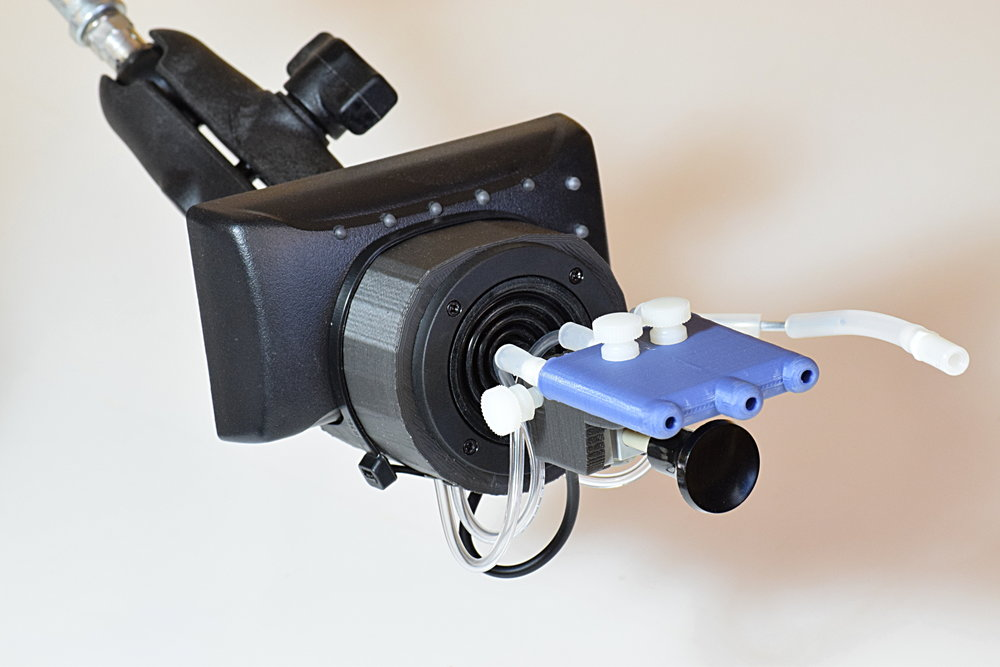
\includegraphics[width=.4\textwidth]{quadstick}
\\
  (a) & (b)
\end{tabular}
%
\caption{(a)~IntegraMouse Plus \cite{INTEGRA} und (b)~QuadStick Gamecontroller \cite{QUADSTICK}}
\label{fig:mund}
\end{figure}

%%%%%%%%% Kopfsteuerung %%%%%%%%%
\subsection{Kopfsteuerung}

Es gibt zwei verschiedene Arten, wie durch den Einsatz des Kopfes mit einem System interagieren werden kann. Zum einen kann eine Kamera verwendet werden, um die Bewegungen des gesamten Gesichtes oder eines bestimmten Teiles davon (\zB des Mundes) zu verfolgen und diese dann anschließend von einem System in die gewünschten Befehle umzuwandeln. Andererseits kann auch eine Vorrichtung am Kopf befestigt werden. Die Interaktion funktioniert durch die Neigungsberechnungen der Sensoren, die Teil der Vorrichtung sind.
\newline \newline
Bei der zweiten Variante könnte beispielsweise ein Stirnband am Kopf befestigt werden, das mit je einem Sensor links und rechts ausgestattet ist. Wird der Kopf in eine Richtung geneigt, wird einer der beiden Sensoren aktiviert. Das Stirnband muss dafür über Bluetooth oder WLAN mit einem Computer verbunden sein, damit eine Software die Bewegungen bzw. Sensoren erkennen und auswerten kann. Damit das Stirnband benutzt werden kann, bedarf es einer individuellen Anpassung, da die seitliche Neigung des Kopfes je nach Benutzer unterschiedlich ist.
\newline \newline
Bei der optischen Variante werden grundlegend zwei Arten der Kopfsteuerung bzw. der Nachvollziehbarkeit der Bewegungen unterschieden:
\begin{itemize}
      \item Gesichtserkennung
      \item Punkteverfolgung
\end{itemize}
\vspace{\baselineskip}
Bei der Gesichtserkennung wird versucht, das Gesicht als Gesamtheit zu erfassen und dieses als Berechnungsgrundlage für die Bewegungen heranzuziehen. Es gibt verschiedene Arten, um die Position des Kopfes zu erkennen. Eine Möglichkeit wäre, die Hautfarbe dazu zu verwenden. Da diese aber von Mensch zu Mensch verschieden ist, ist davon abzuraten, sie als Erkennungsgrundlage heranzuziehen. Des Weiteren sind bei der Berechnung bzw. Filterung viele Schritte notwendig, was mit großem Rechenaufwand verbunden ist. Daher ist eine Mischung aus der haarähnlichen-Gesichtserkennung und dem Camshift-Gesichtstrackingalgorithmus effizienter.
\newline \newline
Für letztere Variante sind grob drei Schritte notwendig \cite{FaceTracking}:
\begin{itemize}
      \item Als Ausgangslage wird der Unterschied vom Haaransatz zum Gesicht verwendet. Hierbei wir das Gesicht in verschiedene Bereiche aufgeteilt.
			\item Danach wird eine Wahrscheinlichkeitsberechnung durchgeführt, damit erkannt werden kann, ob es sich bei den einzelnen Pixeln um den Haaransatz oder das Gesicht handelt.
			\item Abschließend kann auf Grund der Berechnung das Gesicht erkannt werden.
\end{itemize}
\vspace{\baselineskip}
Bei der Punkteverfolgung wird ein bestimmter Teilbereich des Gesichtes fokussiert, der die Bewegungsgrundlage des gesamten Kopfes darstellt. Naizhong und Jing \cite{MouthChinaControl} haben einen Algorithmus entwickelt, der die Mundbewegungen als Grundlage für die Kopfbewegungen verwendet. Dafür wird eine Kamera für den Videoinput verwendet. In der Analyse können die verschiedenen Eingabebefehle unterschieden werden. So ergibt beispielsweise ein Kopfschütteln nach links einen Linksklick oder ein zweimaliges Kopfschütteln nach rechts einen rechten Doppelklick \cite{MouthChinaControl}.
\newline \newline
Für den Benutzer gibt es einige Punkte, die vor und während der Interaktion ausschlaggebend für eine optimale Verwendung sind. Ähnlich wie bei der Augensteuerung in Abschnitt ~\ref{cha:Augensteuerung} muss auch hier das System vorab kalibriert werden, um eine reibungslose Interaktion zu ermöglichen. Des Weiteren gilt es zu beachten, dass keine störenden Lichtquellen auf das Gesicht fallen und ein möglichst frontaler Blick in die Kamera erfolgt \cite{MouthChinaControl}.


%%%%%%%%% Fußsteuerung %%%%%%%%%
\subsection{Fußsteuerung}

Es gibt eine Vielzahl verschiedener Fußsteuerungen. Manche ähneln dem System der Kinnsteuerung und verwenden einen Joystick, um beispielsweise Mausbewegungen zu erzeugen. Darüber hinaus werden verschiedene Tasten für die Auswahl bestimmter Elemente genutzt. Andere wiederum verwenden einen zusätzlichen Schuh bzw. eine Halterung, um die Fußbewegungen zu messen.
%
%
\begin{figure}
\centering\small
\setlength{\tabcolsep}{0mm}	% alle Spaltenränder auf 0mm
\begin{tabular}{c@{\hspace{0mm}}c} % mittlerer Abstand = 12mm
  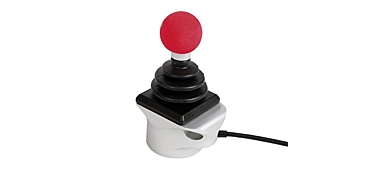
\includegraphics[width=.47\textwidth]{fruewald_joystick} &
  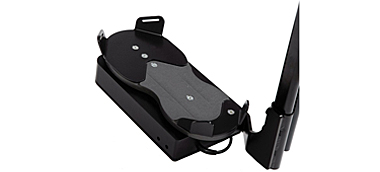
\includegraphics[width=.47\textwidth]{fruehwald_pedal}
\\
  (a) & (b)
\\[7pt]	%vertical extra spacing (4 points)
  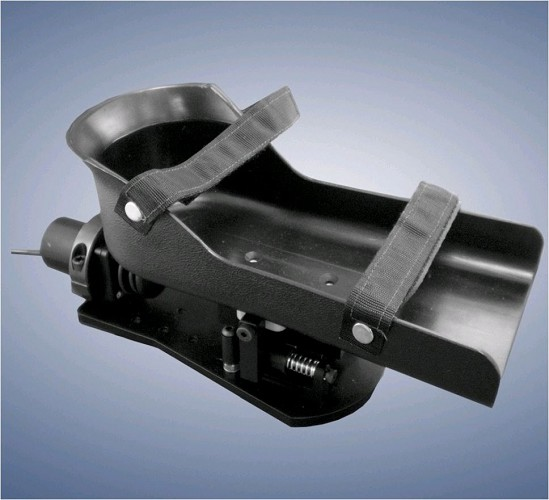
\includegraphics[width=.27\textwidth]{hidrex_pedal}
\\
  (c)
\end{tabular}
%
\caption{(a)~Früwald Joystick \cite{FRUEHWALD}, (b)~Frühwald Fußsteuerung \cite{FRUEHWALD} und (c)~Hidrex Fußsteuerung \cite{HIDREX}.}
\label{fig:foot}
\end{figure}
%
%
\newline \newline
Wie in Abb.~\ref{fig:foot}(a) zu sehen ist, kann ein gewöhnlicher Joystick, der auch mit dem Kinn bedienbar ist, ebenfalls mit dem Fuß bedient werden. Der Benutzer bewegt den Joystick in die gewünschte Richtung und kann damit beispielsweise die Fahrtrichtung eines Rollstuhls oder die Mausbewegung am Computer steuern. Die Fußsteuerung bzw. das Fußpedal (Abb.~\ref{fig:foot}(b)) des Unternehmens Frühwald%
\footnote{https://www.fruehwald.net/}
%
kann durch unterschiedlich starke Druckausübung gesteuert werden \cite{FRUEHWALD}. 
\newline \newline
Bei der in Abb.~\ref{fig:foot}(c) dargestellten Fußsteuerung der Firma Hidrex%
\footnote{http://www.hidrex.de/}%
, handelt es sich um einen Schuhhalter, der als Joystick funktioniert. Die Bedienung ist ähnlich der eines herkömmlichen Joysticks. Der Fuß muss in die gewünschte Richtung gezogen bzw. bewegt werden, um einen Bewegungsablauf nachvollziehen zu können.
%
\newline \newline
Wie die einzelnen Systeme die verschiedenen Gesten in eine Bewegung umwandeln, ist von System zu System verschieden. Häufig findet ein joystickähnliches Element für die Bewegungsrichtung Verwendung. Zusätzliche Tasten helfen bei der Auswahl von gewünschten Symbolen oder Elementen.

%%%%%%%%%%%%%%%%%%%%%%% Muskelsteuerung %%%%%%%%%%%%%%%%%%%%%%%%%%%
\section{Muskelsteuerung}

Bei der Muskelsteuerung wird das Zusammenziehen eines Muskels oder bestimmter Muskelpartien verwendet, um so mit einem Computer interagieren zu können.
\newline \newline
Der Großteil der Muskelsteuerungssysteme nützt zur Messung der Signale das Prinzip der Elektromyografie (EMG). Bei einer EMG-Schnittstelle handelt es sich um die Messung der Muskelkontraktionen. Zusätzlich muss diese Messung mit einer Software für die gewünschten Interaktion verknüpft werden. Die Voraussetzung an den Benutzer besteht lediglich darin, die ausgewählten Muskelpartien selbstständig anzuspannen bzw. zu aktivieren. Im Zusammenhang mit der Muskelsteuerung kommt die Oberflächenelektromyografie (sEMG, englisch für Surface Electromyography) zum Einsatz. Hierbei werden die Elektroden, die für die Messung der Signale ausschlaggebend sind, an der Hautoberfläche angebracht. Mit Hilfe der Elektroden können die myoelektrischen Signale, die die Muskeln produzieren, gemessen und in einem späteren Schritt als bestimmte Interaktion interpretiert werden \cite{EmgDefinition}.
\newline \newline
Abb.~\ref{fig:MyoAblaufOhr} zeigt die einzelnen Schritte, die das Signal im System durchläuft, um am Ende die Interaktion mit einem Computer zu ermöglichen. In der Studie von Barszap, Skavhaug und Joshi \cite{MyoOhr} werden zwei Frequenzbänder verwendet, um eine X- und Y- Richtung des Mauszeigers zu ermöglichen. Zieht sich der Muskel zusammen, so werden alle messbaren Signale erfasst und die relevanten herausgefiltert. Anschließend werden die Signale in zwei Partien aufgeteilt und durch zwei separate Bandpassfilter geschickt. \newline
Dadurch werden die gewünschten Signale bzw. Frequenzen erneut gefiltert und angepasst. Danach werden die beiden Signale in einen Wert zwischen 0 und 100 umgerechnet, der die Ausprägungsstärke in Prozent der jeweiligen Koordinate repräsentiert \cite{MyoOhr}.
\newline \newline
Damit ein Benutzer durch den Einsatz von myoelektrischen Signalen mit einem Computer interagieren kann, müssen zu Beginn die richtigen Positionen für die Anbringung der Elektroden gefunden werden.  
\newline \newline 
Es gibt verschiedene Ansätze, wie die Kalibrierung im Detail aussehen kann. Folgendes Beispiel bezieht sich auf eine Studie von Vernon und Joshi \cite{MyoTraining}.
%
%
\begin{figure}
\centering
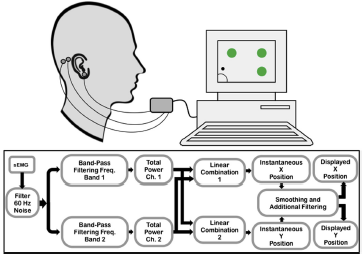
\includegraphics[width=.5\textwidth]{MyoAblaufOhr}
\caption{EMG Signalverarbeitung \cite{MyoOhr}}
\label{fig:MyoAblaufOhr}
\end{figure}
%
%
\begin{figure}
\centering\small
\setlength{\tabcolsep}{0mm}	% alle Spaltenränder auf 0mm
\begin{tabular}{c@{\hspace{15mm}}c} % mittlerer Abstand = 12mm
  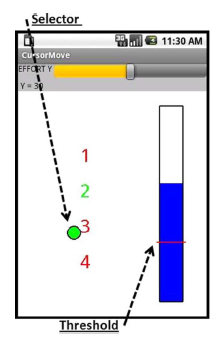
\includegraphics[width=.28\textwidth]{MyoTraining1} &
  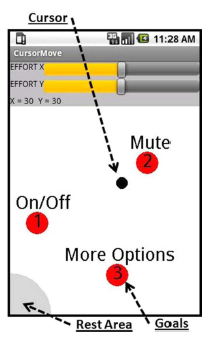
\includegraphics[width=.28\textwidth]{MyoTraining2}
\\
  (a) & (b)
\end{tabular}
%
\caption{Trainingsoberflächen: \newline
(a)~1D-Steuerung \cite{MyoTraining} und (b)~2D-Steuerung \cite{MyoTraining}}
\label{fig:MyoTraining}
\end{figure}
%
%
\newline
Die Elektroden werden an der vermuteten Stelle der zu messenden Muskeln angebracht und mit dem Computer verbunden. Auf dem Bildschirm ist das aktuelle sEMG-Signal zu sehen. Beinhaltet das Signal viele Störfaktoren, das sog. Rauschen, müssen die Elektroden gereinigt oder neu positioniert werden. Ist die optimale Position gefunden worden, muss das System an die individuellen Muskelkontraktionen des Anwenders angepasst werden. Bei diesem Schritt muss der Benutzer die ausgewählten Muskeln über einen Zeitraum von einigen Sekunden so fest wie möglich anspannen, um die maximale Frequenz bzw. Leistung erfassen zu können. Als nächstes werden beim Benutzer zwei verschiedene Testphasen durchgeführt. Der erste Test (Abb.~\ref{fig:MyoTraining}(a)) dient dazu, ein Bewusstsein zu entwickeln, wann und wie stark der gewünschte Muskel angespannt werden soll. Der grüne Punkt auf dem Display bewegt sich je nach Anspannung durch die verschiedenen Stufen und soll auch durch Entspannen wieder zur Ausgangslage gebracht werden. Bei dem zweiten Test, der in Abb.~\ref{fig:MyoTraining}(b) dargestellt ist, handelt es sich um eine zweidimensionale Überprüfung. Hier soll der Cursor in X- und Y-Richtung bewegt werden. Dies geschieht ebenfalls durch An- und Entspannung der einzelnen Muskeln. Beide Versuche bauen auf dem Trial und Error Prinzip auf. Der Benutzer muss also durch mehrere Versuche zur richtigen bzw. besten Lösung kommen. Ist der Anwender mit beiden Trainings vertraut, kann mit der gewünschten Interaktion mit dem Computer begonnen werden. Diese ist auf dem selben Prinzip aufgebaut, allerdings gibt es unterschiedliche Oberflächen, Anordnungen der Elemente und Unterscheidungen in der Aufgabenstellung selbst \cite{MyoTraining}.
\newline \newline
Abb.~\ref{fig:MyoBand} zeigt das Armband des Unternehmens Myo%
\footnote{https://www.myo.com/}
%
. Dieses verwendet die myoelektrischen Signale des Armes, um durch verschiedene Gesten mit dem Computer interagieren zu können. Zu den fünf vordefinierten Gesten zählen \zB das Bilden einer Faust oder Wischgesten. Es können aber auch eigene Gesten definiert bzw. programmiert werden. Zum einen können die vordefinierten Gesten durch die Einberechnung von Armbewegungen erweitert werden, zum anderen gibt es die Möglichkeit neue Gesten zu erstellen, da der Zugriff auf die rohen EMG-Daten möglich ist \cite{myoBand2}.%
\newline \newline \newline 
Damit ein Computer mit Hilfe von Muskelkontraktionen gesteuert werden kann, ist ein aufwendiger und gut überlegter Algorithmus notwendig, um die erfassten Signale in das gewünschte Ergebnis zu transferieren. Vor der Interaktion müssen wie beschrieben einige Schritte durchlaufen werden, um das System an das Individuum anzupassen und um ein Bewusstsein für die Muskelsteuerung zu erlangen.
%
%
\begin{figure}
\centering
\includegraphics[width=.3\textwidth]{MyoBand}
\caption{Myo-Armband \cite{myoBand}.}
\label{fig:MyoBand}
\end{figure}
%
%

%%%%%%%%%%%%%%%%%%%%%%% Gehirnaktiviät %%%%%%%%%%%%%%%%%%%%%%%%%%%
\section{Steuerung durch Gehirnaktivität}

Dieser Abschnitt beschäftigt sich mit der Schnittstelle zwischen dem Gehirn und dem Computer. In der Literatur wird in diesem Zusammenhang von Brain-Computer-Interface (BCI) gesprochen. Ziel ist es, eine direkte Verbindung der beiden Komponenten für eine Interaktion herzustellen. Das BCI liest die Wellen, die vom Gehirn an den verschiedensten Stellen produziert werden ein und übersetzt diese Signale in Befehle, damit mit einem Computer interagiert werden kann \cite{BRAIN}.
\newline \newline
Es gibt verschiedene Aufnahmetechniken von BCIs:
\begin{itemize}
      \item Invasiv
      \item Teilweise invasiv
			\item Nicht invasiv
\end{itemize}
\vspace{\baselineskip}
Invasive Gehirn-Computer-Schnittstellen werden direkt im menschlichen Gehirn durch eine Operation eingesetzt. Es können hier einzelne oder mehrere Einheiten in verschiedenen Bereichen des Gehirns platziert und anschließend angesprochen werden. Diese Systeme weisen die höchste Qualität auf, bringen aber durch die Operation gewisse Risiken mit sich.
Bei teilweise invasiven BCI-Systemen werden die Einheiten nicht direkt in den Gehirnzellen sondern im Schädel eingesetzt, allerdings können sie daher die Signale etwas schlechter empfangen. Bei nicht invasiven Systemen handelt es sich um die sicherste und kostengünstigste Variante auf Kosten von schwächerem Gehirnsignalempfang. Die Signale werden über Elektroden empfangen, die am Kopf befestigt werden. Für diese Technik werden meist mit Hilfe eines Elektroenzephalografen (EEG) die neuronalen Wellen des Gehirns gemessen \cite{BRAIN}.
\newline \newline 
Die neuronale Aktivität des Gehirns ist ausschlaggebend für die Messung. Daher ist es wichtig, die verschiedenen Signale, die ein EEG misst, kurz darzustellen \cite{BRAIN}:
\begin{itemize}
      \item Delta Signal: Hierbei handelt es sich um die langsamsten Wellen mit einer Frequenz zwischen 0.5 und 3.5 Hz, die während des Schlafens oder im komatösen Zustand auftreten.
      \item Theta Signal: Es handelt sich hierbei um Wellen, die beispielsweise während des Träumens vorkommen. Die Frequenzen werden in einem Bereich zwischen 3.5 und 7.5 Hz gemessen.
			\item Alpha Signal: Dies sind langsamere Wellen, die beim Entspannen auftreten (Frequenzen zwischen 7.5 und 12 Hz).
			\item Beta Signal: Diese Wellen sind oft mit Anstrengung, wie beispielsweise des Lösens einer mathematischen Aufgabe, verbunden und liegen in einem Bereich zwischen 12 und 30 Hz.
      \item Gamma Signal: Je größer hier die Amplitude ist, desto mehr Stress, Angst oder Panik erlebt die Personen (alle Frequenzen ab 31 Hz).
\end{itemize}
\vspace{\baselineskip}
Je nach Anwendungsbereich können verschiedene Signale verwendet werden. Für eine Interaktion mit einer Person, die sich nicht in einem komaähnlichen Zustand befindet, sind alle Signale ab einer Stärke von 3.5 Hz relevant.
\newline \newline
%
%
\begin{figure}
\centering
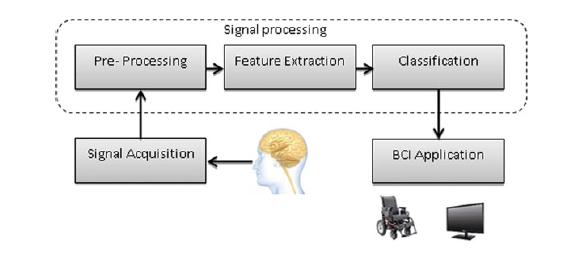
\includegraphics[width=.9\textwidth]{BCI}
\caption{BCI Signalverarbeitung \cite{BRAIN}.}
\label{fig:BCI}
\end{figure}
%
%
Für den gesamte Ablauf, der nötig ist, um eine Gehirn-Computer-Schnittstelle zu erstellen sind, wie in Abb.~\ref{fig:BCI} veranschaulicht, sind grob drei Schritte notwendig \cite{BRAIN}:
\begin{itemize}
      \item Signalerfassung: Im ersten Schritt werden die elektrischen Signale von der Kopfhaut oder der Oberfläche des Gehirns erfasst.
      \item Signalverarbeitung: Da die diese Signale in der Regel sehr schwach sind, werden sie als nächstes verstärkt und von Störvariablen gereinigt. Danach durchlaufen die Signale einen Übersetzungsalgorithmus, damit die Absichten des Benutzers erkannt werden können.
			\item Signalinterpretation: Im letzten Schritt müssen die Daten von einem Programm bzw. einer Software so interpretiert werden, damit diese für eine Computerinteraktion verwendet werden können.
\end{itemize}
%
%
\vspace{\baselineskip}
\vspace{\baselineskip}
\vspace{\baselineskip}
%bild epoc
%beschreibung epoce
\begin{figure}
\centering
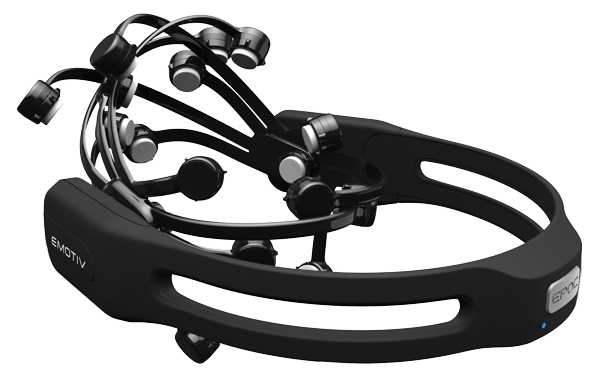
\includegraphics[width=.5\textwidth]{epoc}
\caption{Emotiv EPOC+ \cite{epoc}}
\label{fig:epoc}
\end{figure}
\vspace{\baselineskip}
Abb.~\ref{fig:epoc} zeigt das EPOC+ des Unternehmens Emotiv%
\footnote{https://www.emotiv.com}
%
. Es werden 14 EEG Kanäle genutzt, um bestmögliche Signale zu empfangen. Das Headset wird über WLAN mit einem Computer verbunden und zeigt die Gehirnaktivität in Echtzeit. Durch erhöhte Gehirnaktivität in bestimmten Areal können Charaktere in einem Computerspiel oder ein ferngesteuerter Hubschrauber gesteuert werden. Interaktionen durchgeführt werden. Über den Zugang zu den rohen EEG Daten, kann eine  Software programmiert werden, die eine individuelle Interaktion mit einem System ermöglicht \cite{epoc}. 
\newline \newline
Um als Benutzer einen Computer mit Hilfe von Gehirnaktivität steuern zu können, muss das System vor der Interaktion individuell angepasst werden. Als mögliche Kalibrierungsmethode kann ein Mauszeiger gedanklich mitverfolgt werden, während dieser sich bewegt. Der Benutzer soll sich hierbei vorstellen, er würde die Bewegung mit der Hand oder dem Arm ausführen. Je nach Person zeigt sich die Anstrengung in dem motorischen Teil des Gehirns unterschiedlich stark und das System wird dahingehend angepasst. Im nächsten Schritt wird erneut ein Mauszeiger gedanklich mitverfolgt. Allerdings erscheint ein zweiter Cursor, der auf Grundlage der bereits erhobenen Daten den momentanen Stand aufzeigt. Diese zwei Schritte werden mehrmals durchgeführt, um ein optimales Ergebnis zu erzielen. Neben der Mausbewegung kann auch ein Mausklick simuliert werden. Die Auswahl eines Menüpunktes kann beispielsweise so funktionieren, dass ein Menüpunkt hervorgehoben wird. Hat der Anwender sich für einen bestimmten entschieden, muss er sich besonders darauf konzentrieren bzw. die Gehirnbereiche müssen eine erhöhte Aktivität aufweisen \cite{BrainInt}.
\newline
Darüber hinaus muss nicht nur der Benutzer an das System angepasst werden, sondern auch umgekehrt. Bei jeder Interaktion kann das System die Eigenheiten des Individuums besser erfassen, korrigiert Fehler und kann sich durch das ständige Mitlernen verbessern. 
\newline \newline
Die Interaktion mit Hilfe der Messung der Gehirnaktivität ist im Gegensatz zu den zuvor beschrieben Methoden eine komplexere und aufwändigere Eingabemethode. Auch die Kalibrierung und das Training des Systems erfordern einen höheren Aufwand.
